\chapter{Algebro-Geometric Background}\label{chap1}

\section{Algebraic Varieties: Affine and Projective}\label{chap1:sec1}%sec 1.1

\textbf{a)}~ We\pageoriginale consider the affine $n$-space $K^n$ over an algebraically
  closed field $K$. An algebraic set $H$ in $K^n$ is, by definition,
  the set of common zeros $(x) = (x_1,\ldots, x_n)  \in   K^n$ of a
  family of polynomials $(F_\alpha ), F_\alpha \in  K [X_1,\ldots,
    X_n]$, or equivalently, of polynomials in an ideal $\mathscr{O}$
  of $K [X_1,\break\ldots,X_n]$. A finite union of algebraic sets, and an
  arbitrary intersection of algebraic sets are easily seen to be
  themselves algebraic sets so that, in $K^n$, we have a topology,
  called the Zariski topology, whose closed sets are precisely the
  algebraic sets in $K^n$. These algebraic sets are often called the
  closed sets of $K^n$ or the \textit{affine algebraic sets.} 

  Given an affine algebraic set $H \subset K^n$ we define the \textit{
    ideal of $H$ } $\mathcal{J}(H)$, as  
  $$
  \mathcal{J}(H) = \left\{ F \in K [X_1,\ldots, X_n] : F (x) = 0~
  \forall (x) \in  H \right\}. 
  $$

  The \textit{affine ring of $H$}, or the \textit{coordinate ring of
    $H$} is, by definition, the ring $K [X_1,X_2, \ldots, X_n] \bigg /
  \mathcal{J} (H) = K[H]$. We remark that the elements of $K[H]$ are
  functions on $H$ with values in $K$, in a natural manner.  

  We say that an affine algebraic set $H$ is \textit{ irreducible } if
  it is non-void and is \textit{ not } the union of two proper
  algebraic subsets; it is not difficult to see that $H$ is
  irreducible $\Leftrightarrow \mathcal{J}(H)$ is a prime\pageoriginale ideal of $K
  [X_1,\ldots,X_n] \Leftrightarrow K[H]$ is a domain. An irreducible
  algebraic set is often called a \textit{Variety} (We may also use
  the term sometimes for algebraic sets). One can show that any algebraic set
  $H$ in $K^n$ can be written, in a unique manner, as a finite
  irredundant union of varieties in $K^n$ 

\textbf{b)}~ Let $k$ be a subfield of $K$ and $V$ an algebraic set in
  $K^n$. We say that $V$ is defined over $k$, or that $k$ is a
  \textit{ field of definition } for $V$ if $\mathcal{J}(V)$ admits a
  set of generators in $k[X_1,\ldots, X_n] \subset
  K[X_1,\ldots,X_n]$, or equivalently, if $\exists$ a finite type
  $k$-algebra $k[x_1,\ldots, x_n]$ such that $K[V] \simeq
  k[x_1,\ldots,x_n] \otimes_k K$. As, by the basis-theorem of Hilbert,
  $\mathcal{J}(V)$ admits finitely many generators in
  $K[X_1,\ldots,X_n]$, any algebraic set in $K^n$ admits a field of
  definition which is of finite type over the prime field. 

  Consider a variety $V$ in $K^n$; then $K[V]$ is a domain. Its field
  of fractions is called the \textit{function field} (or the rational
  function field) of $V$ and denotes by $K(V)$. If $k$ is any subfield of $K$ which is a
  field of definition for $V$, then one defines the $k$-ideal of $V$
  by 
  $$ 
  \mathcal{J} (V) = \left\{ G  \in   k [X_1,\ldots, X_n] : G(x) = 0~
  \forall (x)\in V \right\} 
  $$
  and the $k$-ring of functions on $V$ by
  $$ 
  k[V] = k [X_1,\ldots, X_n]/ \mathcal{J}_k (V):
  $$
  one sees that $k[V]$ is again a domain, and further that
  $k[V]\otimes _k \bar{k}$, ($\bar{k}= $ the algebraic closure of $k$)
  is also a domain. One can check that this\pageoriginale last fact is equivalent to
  the fact that the $k$-function field $k(V)=$ the field of fractions
  of $k[V]$ is a \textit{regular} extension of $k$ (i.e. is separately
  generated over $k$ and $\bar{k} \cap k(V) = k$) (cf.~\cite{4}) 

  Let $V$ be a variety in $K^n$ and $k$ a field of definition for
  $V$. Consider a point $ (y) = (y_1,\ldots, y_n) \in V$ and the
  homomorphism $k[X_1,\ldots, X_n] \rightarrow k[y_1,\ldots, y_n]\subset
  K$ defined by $X_i \to y_i$. By the definition of $k[V]$ this
  homomorphism admits a factorization  
\[
\xymatrix{k [X_1 ,\ldots, X_n] \ar[dr]\ar[rr] && k[y_1,y_2, \ldots,
    y_n]\subset K\\ 
  & k[V] \ar[ru]_\varphi& 
}
\]
  We say that the point $(y)$ is a \textit{generic point} for $V$ over
  $k$ if $\varphi$ is an isomorphism (note that the irreducibility of
  $V$ over $k$ is necessary for the existence of such a point). One
  can show that a generic point for $V/k$ exists if $K$ has infinite
  transcendence degree over $k$.  

  On the other hand, let $k$ be a subfield of $K$ and $(x) \in K^n$
  such that $k(x) = k(x_1,\ldots, x_n)$ be a regular extension of
  $k$. If one defines an ideal $\mathcal{J}$ in $k[X_1,\ldots,X_n]$ by
  $\mathcal{J} = \left\{ F  \in   k[X_1,\ldots,X_n] : F(x) = 0
  \right\}$ then the polynomials of $\mathcal{J}$ define a variety
  $V$ in $K^n$ such that 
  \begin{enumerate}[(i)]
  \item $(x)$\pageoriginale is a generic point of $V/K$
  \item $k[V]\simeq k[X_1,\ldots,X_n]/ \mathcal{J}$
  \item $\mathcal{J}(V) = \mathcal{J}_k (V). k[X_1,\ldots, K_n]$
    
    \qquad $= \mathcal{J}. K[X_1,\ldots,X_n]$
  \end{enumerate}

  $V$ is called the \textit{locus} of the point $(x)$ in $K^n$.

  \begin{example*}%exmpl
    $k = \mathcal{Q}, K=\mathbb{C}, (x) =(e^2, e^3)$; then the locus of
    $(x)$ is the curve $X^3_1- X_2^2 = 0$. 
  \end{example*}

\noindent\textbf{c) Dimension}

Let $V$ be an (irreducible) variety in $K^n$ and $K(V)$ the function
field of $V$. Then $K(V)$ is of finite type over $K$; its
transcendence degree over $K$, which is finite, is called the
\textit{dimension} of the variety $V$. Once has then the classical  
 
\begin{theorem*}%thm 
  dimension of $V$= the Krull dimension of $K[V]$.
\end{theorem*}

We remark that the above equality makes the definition of the
dimension of $V$ more intuitive: it says precisely that $\dim$. $V$ is
the maximum length of strictly increasing chains of subvarieties of
$V$. 

Any point $P  \in   K^n$ is a variety of dimension 0; more precisely
we have: a variety $V \subset K^n$ has dimension 0 
\begin{align*}
  & \Leftrightarrow  \text{ V is  a  point }\\
  &\Leftrightarrow  \mathcal{J} \text{ (V) is  a  maximal  ideal }
\end{align*}

(This is essentially the Hilbert-Zero-Theorem).
\begin{prop*} %Propo
  A\pageoriginale variety $V$ in $K^n$ ban dimension $(n-1)$  
  $$
  \Leftrightarrow \mathcal{J} (V)\text{ is principal}
  $$
\end{prop*}

\begin{proof} %pro
  $\Rightarrow: V$ has dimension $(n-1)$ implies that $\mathcal{J}
  (V)=0$. Thus $\exists$ a non-zero polynomial in $\mathcal{J}(V)$ and
  hence a non-zero irreducible polynomial $F$ in
  $\mathcal{J}(V)$. Then $0 \neq (F) \subset \mathcal{J} (V)$; as
  $(F)$ and $\mathcal{J}(V)$ are both prime ideals, and as $\dim K
  [V]=$ coheight $\mathcal{J} (V)= (n-1)$, and $ \dim K
  [X_1,\ldots,X_n] = n$ one gets \textbf{$(F) = \mathcal{J}(V)$}. 
\end{proof}

$\Leftarrow $: If $\mathcal{J}(V) = (F)$, one has $K[V] = K
[x_1,\ldots ,x_n]$ with  $F(x_1,\ldots, x_n)$ $=0; F$ involves at least
one variable, say $X_n$, non-trivially. Thus, $x_n$ is algebraic on
$K(x_1,\ldots,x_{n-1})$. On the otherhand, if $\exists G \neq 0$ in
$x_{11},\ldots, x_{n-1}$ such that $G (X_1,\ldots,X_{n-1}) = 0$ then $G
\in (F)$; as $F$ involves $X_n$ and $G$ does not, this is
impossible. Therefore $X_1,\ldots ,X_{n-1}$ are algebraically
independent over $K$. \hfill Q.E.D

A variety in $K^n$ of dimension $(n-1)$ is called a
\textit{hypersurface} of $K^n$; the above proposition says merely that
hypersurfaces are precisely those varieties which admit a single
``equation''. 
 
\medskip
\noindent\textbf{d) The concept of an ``abstract variety''} 
	
Let $V$ be an algebraic set in $K^n \, j$ for any $P\in V$, there is a
maximal ideal $\mathcal{M}_P$ of the coordinate ring $K[V]$, namely,
the ideal of functions in $K[V]$, null at $P$. The local ring
$\mathscr{O}_P = K[V]_{\mathcal{M}_P}$ is called the \textit{local
  ring $\mathscr{O}_P$ of $P$} (or of $V$ at $P$). More generally, if
$W$ is an irreducible subvariety of $V$, then $\exists$ a\pageoriginale prime ideal
$\mathcal{P}$ of  $K[V]$, namely, the ideal of functions in $K[V]$
null on $W$: the local ring  $K[V]_{\mathcal{P}}$ is called the
\textit{local ring $\mathscr{O}_W$  of $W$ in $V$}. By the Hilbert
Zero theorem, for any prime ideal $\mathcal{P}$ of $K[V], \exists $ a
subvariety $W$ of $V$ such that $\mathscr{O}_W= K[V]_{\mathcal{P}}$. 
 
 It is not difficult to see that the pairs $(P,\mathscr{O}_P)_{P \in
   V}$ form, in a natural way, a subsheaf of the sheaf of functions on
 $V$ in to $K_p$: thus, we get, what is called a \textit{ringed space},
 $(V,\mathscr{O})$. A pair $(X,\mathscr{O}_X$) where $X$ is a
 topological space space and $\mathscr{O}_X$ a given a sheaf of rings
 on $X$, is called a ringed space : here, we shall be interested only
 in the case where all the stalks $\mathscr{O}_x, x \in X$, are local
 rings; thus we will assume this additional condition always
 satisfied). If $(X,\mathscr{O}_X), (Y,\mathscr{O}_Y)$ are two ringed
 spaces, a \textit{morphism} $(X,\mathscr{O}_X)
 \overset{f}{\rightarrow} (Y,\mathscr{O}_Y)$ is a pair
 $(u,\theta)$ where $u$ is a continuous map of topological spaces
 and $\theta$ is a morphism (of sheaves of local rings over $Y$)
 $\mathscr{O}_Y \rightarrow$  $u_* (\mathscr{O}_X) (u_* (\mathscr{O}_X)$
 is the ``direct image'' of $\mathscr{O}_X$ under $u) \theta$; is
 essentially a ``nice collection'': $\theta = (\theta_x)_{x
   \in X}$, where $\theta_x: \mathscr{O}_{u(x)} \rightarrow
 \mathscr{O}_x$ is a homomorphism of local rings (For details see
 EGA. Ch. I). 
    
Our ringed spaces can thus be made objects of a category.
\begin{defi*} %Def
  An \textit{(abstract) prevariety} $X$ over $K$ is a ringed space
  $(X,\mathscr{O}_X)$ such that there is a finite open covering
  $(U_i)_i$ of the underlying space $X$ with the following
  property: 
\end{defi*}

$\forall i$, there is an affine variety $V_i$ over $K$ such that the
restricted ringed space $(U_i ,\mathscr{O}_X \mid U_i)$ is isomorphic
to the ringed space $V_i,\mathscr{O}_{Vi}$ of the affine variety $V_i$. 

The\pageoriginale notions of irreducibility, rational maps, morphisms, subs.,
products, fields of definition and a generic point of an irreducible
prevariety over a field of 
definition, can all be easily carried over. In particular, one
defines the \textit{diagonal map} $\Delta_X : X
\rightarrow X\times X$ for a prevariety $X$. 

\begin{defi*}%def
  We say that a prevariety $X$ is a \textit{ variety } if the
  diagonal map $\Delta_X$ is closed  
\end{defi*}

We remark that this condition is analogous to the Hausdorff axiom on a
topological space. 

In the category of varieties isomorphisms will be often called
\textit{ biregular maps }. We say that a morphism $f$ biregular at a
point $x \in X$, if the stalk-map $\mathscr{O}'_{f(x)} \rightarrow
\mathscr{O}_{x}$ defined by $f$ is an isomorphism. One can show that
biregularity at $x$ implies biregularity in a neighbourhood of $x$. 
 
\medskip
\noindent \textbf{e) Projective Varieties}

Let $K$ be an algebraically closed field. The \textit{ projective
  $n$-space} $\mathbb{P}_n (K)$ over $K$  is, by definition, the
quotient of $K^{n+1} -(0)$ for the action of $K^*$ by scalar
multiplication. An algebraic set in $\mathbb{P}_n (K)$ is the image of
an algebraic cone in $K^{n+1}$. Any point in
$\mathbb{P}_n(K)$ can be represented, upto a scalar multiplication, by
an $(n+1)$-tuple $(x_0,\ldots, x_n)$, the $x_i \in K$, \textit{ not }
all zero. Such a representation is called a system of (homogeneous)
coordinates $(x)$ for that point. An algebraic set in $\mathbb{P}_n
(K)$ is then the set of points $(x)\in \mathbb{P}_n (K)$ such that
$F_{\alpha} (X) = 0 $ for a family of homogeneous polynomials
$(F_{\alpha}),F_{\alpha} \in K [X_0 ,\ldots , X_n]$.\pageoriginale
One can again define a topology on $\mathbb{P}_n (K)$ (the
Zariski topology) whose closed sets are the algebraic sets in
$\bP_n(K)$. One again defines as before the notion of a projective
variety in $\bP_n 
(K)$. For  any algebraic set $V$ in $\mathbb{P}_n (K)$, one defines
the homogeneous ideal $\mathscr{H} \mathcal{J}(V)$ of $V$ as the ideal
generated by all homogeneous polynomials in $K[X_0,\ldots, X_n]$
vanishing on $V$, and the homogeneous coordinate ring or the
\textit{graded ring} of $V$ as the quotient $K[X_0,\ldots,X_n] /
\mathscr{H} \mathcal{J} (V)$. 

A projective algebraic set $V$ is a variety $\Longleftrightarrow
\mathscr{H} \mathcal{J}(V)$ is a prime ideal \textit{ not } containing
the ideal $(X_0,\ldots,X_n)$. One defines as before the notion of a
(homogeneous) generic point for a projective variety $V$, over a
subfield $k$ of $K$. 
   
One has a bijective map of $K^n$ onto the open set $X_0 \neq 0$ of
$\mathbb{P}_n (K)$ given by $(y_1,\ldots,y_n)  \longmapsto
(1, y_1,\ldots,y_n)$. This map is a homeomorphism on to its
image $X_0 \neq 0$, which we will call $K_0$. The hyper-plane
$H_0$,given by $X_0 = 0$,is  
called the hyper-plane at infinity for the affine subspace
$K_0$. Similarly we have hyperplanes $H_i \equiv X_i =0$, whose
complements $K_i$ are affine,$1\leq i\leq n$. Clearly $\mathbb{P}_n
(K) = \bigcup \limits^{n}_{i=0} K_i$. If $U$ is an affine algebraic
set in $K^n$. given by prescribing a system of generators for $K[U],
K[U] = K[X_1,\ldots,X_n]$ say, we get an imbedding of $U$ as a subset
of $K_0$, hence of $\mathbb{P}_n(K)$. The closure of $U$ in
$\mathbb{P}_n (K)$ is called a \textit{ projective closure } of $U$. 

Let\pageoriginale $V$ be a projective variety in $\mathbb{P}_n (K)$ then $V= \bigcup
\limits^{n}_{i-0} V_i$ 
where $V_i = V \cap K_i = V-H_i$, each $V_i$ as ***** of $K_i$ is an
affine algebraic set. Further, if $K[x_0,\ldots x_n]$ with $x_0 \neq 0$
is the homogeneous coordinate ring of $V$ and if we set $y_i =
\dfrac{x_i}{x_0}, 1\leq i\leq n$ (then the $y_i$ are in the quotient
field of $K[V]$)  then $V_0  = V-H_0$ is an affine variety of affine
ring $A_0 = K[y_1,\ldots,y_n]$ and $V_i, i\ge 1$, if nonvoid, is an
affine variety of affine ring  
$$
A_i = K\left[\dfrac{1}{y_i},\ldots,\dfrac{y_n}{y_i}\right].
$$   

To show that a projective to show variety $V$ is a variety in the
sense of $(\alpha)$, it only remains to show that the diagonal of $V$
is closed; we leave the verifications to the reader. 

Finally, we define the function field of a projective variety $V$ as
the subfield $K(V)$ of the quotient field of $K[V]$ defined by $K (V)
= \Bigg\{ \dfrac{a}{b}: a,b \in K [V], b \neq 0, a,b$ are of the same
degree in the gradation on $K[V]\Bigg\}$  
 
If $V$ is \textit{ not } contained in $H_i$, then one can show that
$K(V)$ is canonically isomorphic to the quotient field of $A_i$ (in
the above notation). 

\begin{theorem}\label{chap1:sec1:thm1} %theom 1.
  A projective variety $V$ is \textit{complete} in the following
  sense: \textit{Every valuation  ring  $\mathscr{O}$ of $K(V)$
    contains some } $A_i$. 
\end{theorem}

\begin{proof}%proof 
  Let $\omega $ be the valuation defined by $\mathscr{O}$ on
  $K(V)$. If $\omega (y_i) \ge 0$ for all $i$, then
  $\mathscr{O}\supset A_0$; otherwise choose an $i$ such that $\omega
  (y_i)$ is minimum; then $\omega (y_i) < 0$ and $\mathscr{O} \supset
  A_i$. 
\end{proof}

\begin{remark*}%emark
  One\pageoriginale can define fields of definition for projective varieties as for
  affine varieties. If $k$ is a field of definition for $V$, one can
  define $k[V]$ as before and $V$ is a finite union at affine
  subvarieties  for which again $k$ is a field of  definition. All our
  computations above go through and the obvious modifications of
  Theorem~\ref{chap1:sec1:thm1} is also valid. 
\end{remark*}

\begin{theorem}\label{chap1:sec1:thm2} %theo 2
  If $V$ is a projective  variety, then for any variety $U$ the
  projection $p$ of $V \times U$ on $U$ is a closed map. 
\end{theorem}  
 
\begin{proof}%proof
  We have to show that for any closed  subset $H$ of $V \times
  U$, $p(H)$ is closed in $U$. We may assume $V,U,H$ all to be
  irreducible. Let then $(y,x) \in V \times U $ be a generic point
  for $H$ over a field of definition $k$ of  $V,U$ and $H$. If $x'\in
  \overline{p(H)}$ then $x'$ belongs  to the locus  of $x$ over $k$ in
  $U$, and  there is a homomorphism (over $k$) $k [x] \xrightarrow{\varphi}
  k [x']$,mapping $x$ on $x'$. As $k[x]
  \subset k (V \times U)$ and as  $K$ is algebraically closed,
  $\varphi$ extends to a valuation ring $R$ of $k(V \times U)$ as a
  homomorphism  $\bar{\varphi}: R \rightarrow K$. By (the  remark
  following) Theorem~\ref{chap1:sec1:thm1}, there  is a system of affine  coordinates
  $z_1,\ldots, z_n$ of $(y)\in V$ such that all  the $z_i$ are in $R$:
  thus  there is a point $(y') \in \mathbb{P}_n (K)$ with affine
  coordinates $(\bar{\varphi} (Z_1),\ldots ,\bar{\varphi} (Z_n))$. But
  as  $k[x', y']\subset k,  k [x,y]\subset k (U \times V)$ and
  $\overline{\varphi}$ is a homomorphism mapping $(x,y)$ on $(x', y')$
  it follows  that $(y',x'$) $\in H$ and \textit{$x' \in p(H)$.} 
\end{proof} 


Finally we also draw the attention of the reader to the fact that the
product of two projective  spaces $\mathbb{P}_n (K),\mathbb{P}_q (K)$
is a projective variety; this is shown by the \textit{Segre imbedding} 
\begin{align*}
  \mathbb{P}_n (K) \times \mathbb{P}_q (K) & \longrightarrow
  \mathbb{P}_{(n+1)(q+1)-1} (k)\\ 
  ((x_i),  (y_j))  &\longmapsto (x_iy_i).
\end{align*} 

\noindent \textbf{f) Dimension Theorems.}\pageoriginale

  If $A$  is a noetherian ring, $x \in A$  and $\mathscr{Y}$a minimal
  prime ideal of $Ax$ then  $ ht \mathscr{Y} \leq i$ (Krull); if $x$ is
  not a zero divisor of $A$, then $ht \mathscr{Y}=1$. 

\begin{enumerate}[1)]
  \item  If $V$ is an affine variety of  dimension $d$ in $K^n$, and
    $H$ a hyper surface in $K^n$, then every component of $V \cap H$
    has dimension  $d$ or $(d-1)$. 
 
    If $H \equiv (f=0), f \in k[X_1,\ldots X_n]$ then $V \cap H$ is
    given by $\bar{f}=0$ in $A=K[V]$ ($\bar{f}$ image of $f$ in
    $K[V]$) and its components are given by the minimal prime ideals
    of $A\bar{f}$ so that our assertion follows by our remark at the
    beginning. 
 
    If $V$ is irreducible and $V \not\subset H$ then the same shows
    that every component of $V \cap H$ had dimension $(d-1)$.  
  \item By an inductive argument one gets that: if $V$ is affine, of
    dimension $d$ and if $H_1, \ldots, H_q$ are hypersurfaces, then
    every component of $V \cap H_1 \cap \cdots  \cap H_q$ has
    dimension $\ge  (d-q)$. 
 \item If $V$ and $W$ are affine algebraic sets in $K^n$ and $C$ a
   component of $V \cap W$ then \textit{$\dim C \ge \dim V+ \dim
     W-n$}. 

   In fact $V \cap W $ is isomorphic in a natural way with $(V \times
   W )\cap \Delta $ in $K^n \times K^n,\Delta $ being the diagonal in
   $K^n \times K^n$, thus our assertion follows  from the facts that
   $\dim (V \times W) = \dim V + \dim W$, that $\Delta $ in $K^n
   \times K^n$ is the intersection of $n$ hyperplanes and $2$) above. 

   We remark  that $3)$ does \textit{not} say that $ V \cap W \neq
   \phi$ even if $\dim V + \dim W-n \ge 0; (e,.g)$ two parallel lines  
   in $K^2$. However we have the following: 
 \item $\mathscr{G} V,W$\pageoriginale are projective varieties in $\bP_n
   (K)$ such that $\dim V+ \dim W-n \ge O$, then $V \cap W \neq \phi$,
   and each component $C$ 
   of $V \cap W $ has dimension $\ge  \dim V + \dim W-n$. 
 
   In fact $V$, $W$ are images of cones $V'$ $W'$ in $K^{n+1}$ has $V'
   \cap W' \neq \phi$ since the origin is in $V' \cap W'$ are both
   cones and as 
   $$
   \dim V' +\dim  W' -(n+1) = \dim V + \dim W -(n-1) > 0
   $$
   there is a ray throughout the origin in $K^{n+1}$ completely contained in 
   $V' \cap W'$, this implies that $V \cap W \neq \phi $ in
   $\mathbb{P}_n (K)$; any component $C$ of $V \cap W $ corresponds to
   a component $C'$ of $V' \cap W'$ so that by 3) 
   \begin{align*}
     \dim C' &\geq  \dim V' +\dim W' -(n+1)\\
     &= \dim V +\dim  W -n +1\\
     \text{ and }  \hspace{2cm}\dim C  & = \dim C' -1 \geq \dim  V +
     \dim W -n 
   \end{align*}  
 \item Let $U$ be an algebraic variety over an algebraically closed
   field $K$. We say that a point $P \in U$ is \textit{ simple } if the
   local ring $\mathscr{O}_p$ of $V$ at $P$ is \textit{ regular.} 
\end{enumerate}

\begin{prop*}%propo
  If $P$ is a simple point on $U$ and $V$ and $W$ are subvarieties of
  $U$ passing  through $P$, then any component $C$ of  $V  W$ passing
  through $P$ has dimension $\ge \dim  V + \dim W -\dim U$.   
\end{prop*}

\begin{proof}%proof
  The question being local we may assume that $U$ is an affine
  variety imbedded in $K^n$ and $V$, $W$ are closed irreducible
  subvarieties of $U$. If $d= codim_{K^{n}} U$ then $\dim U = (n-d)$:
  and $P$ being simple on $U$, the tangent space of $U$ at $P$ is a
  linear subvariety $L$ in $K^n$ of dimension = $(n-d)$. Let $L'$ be a
  linear $d$-dimensional variety transverse to\pageoriginale $L$ and $V'$ be the
  cylinder parallel to $L$ with base $V$ (\textit{locally}, at $P, V'
  \simeq V \times L'$). Then dimension of $V'$ is equal to $(d + \dim
  V)$.  
\end{proof}

\begin{figure}[H]
\centerline{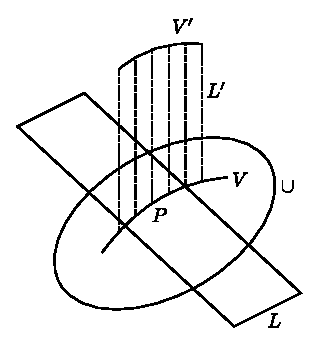
\includegraphics{vol36-figures/fig36-1.eps}}
\end{figure}

 It is not difficult to show that the only component of $ V' \cap U$
 passing through $P$ is $V$. Thus, we have only to show that for any
 component $C$ of  $V' \cap W$ passing  through $P, \dim C \ge
 (\dim V + \dim  W- \dim U)$. 

But by 3) we have:
 \begin{align*}
   \dim  C & \geq \dim  V' + \dim  W -n\\
   &= \dim V + \dim W -(n-d)\\
   &= (\dim  V + \dim W -\dim  U) \tag*{Q.E.D.}
 \end{align*}  
 \hfill{

\noindent\textbf{g) Zariski's main theorem $(ZMT)$.}
  
 A point $P$ on an algebraic  variety $V$ is said  to be
 \textit{normal} of the local ring  $\mathscr{O}_P$ of $V$ at $P$ is
 \textit{ integrally closed }. 
 
 An affine variety $V$ is normal (i.e. \text{ each point}  $P \in V$
 \text{is normal})  $\Longleftrightarrow  K [V]$ is a normal domain.  

If\pageoriginale $V$ is an affine variety and $K[V]$ its coordinate ring then the
integral closure 
$K[V]'$ of $K[V]$ in $K(V)$ is a $K$-algebra of finite type which is
a domain and therefore is the coordinate ring of at affine variety
$V^*$, which is normal; and one has a morphism $V^* \xrightarrow{p} V$
defined in a natural way which is birational and onto. 

We also remark that the same procedure can be adopted in the case of
any arbitrary algebraic variety $V$ (cf. \cite{7}); one has only to
construct pairs of the type $(U^*_i,p_i)$ for an affine open covering
$(U_i)$ of $V$ and patch up. We thus obtain a normal variety $V^*$ and
a birational, onto, morphism $V^*\xrightarrow{p} V$ such that the pair
$(V^*,p)$ is universal for morphisms from normal varieties $V'$ to
$V$. Then $V^*$ is called the \textit{normalisation} of $V$. 

We shall show that if $V$ is projective then $V^*$ is also
projective. If $V$ is a projective variety then its homogeneous
coordinate ring $K[V]$ is a graded domain and its normal closure $B'$
in its quotient field is again a graded domain (is contained in the
quotient-ring $F^{-1}A, F$ the set of homogeneous (non-zero)
elements). Let $B'= \sum\limits_{n \geq 0} B_n'$ be the gradation of
$B'$ ; as above $B'$ is a finite type $K$-algebra. But one cannot
assert that $B'$ is generated over $K$ by homogeneous elements of
degree $1$; however, it is not difficult to see that $\exists~ d  \in
\mathbb{Z}^+$ s.t. $B'' = \sum\limits_{n \geq 0} B'_{nd}$ is a graded
domain, and a finite type $K$-algebra, generated by homogeneous
elements of degree $1$ so that $B''$ defines a projective variety
$V^*$, normal, with a birational, onto regular map
$V^*{\xrightarrow{p}} V$ with finite fibres; so we are through. We
shall now state the following theorem without proof.  

\begin{theorem*}%theo
  Let\pageoriginale $A$ be a domain and $B$ an over-domain which is a finite type
  $A$-algebra, $B = A [x_1,\ldots,x_n]$. Let $p$ be a prime ideal
  in $B$ which is both minimal and maximal in the set of prime ideals
  of $B$ having the intersection $p \cap A$ with $A$. Then if $A'$ is
  the integral closure of $A$ in $B$, one has $B_{p} = A'_{p \cap A'}$.     
\end{theorem*}

\begin{remark*}
  Finiteness conditions on $A$ are \textit{not} needed, as shown by\break
  Grothendieck, or more elementarily, by C. Peskine: ``Une
  generali\-sation du main th\'eor\`eme de Zariski'', Bull,
  Soc. Math. 1966. 
\end{remark*}

\begin{coro*}%Coro
  If $A$ is integrally closed in $B$ then
  $$
  B_{p} = A_{p \cap A}.
  $$ 
\end{coro*}

Geometrically the above theorem says that if $f : Y \to X$ is a
generically surjective (i.e., dominant) morphism of irreducible
varieties and if $y \in Y$ is isolated in the fibre $f^{-1}(f(y))$,
then $\mathscr{O}_{y}$ is a ring of fractions of some finite extension
of $\mathscr{O}_{f(y)}$. If, in addition, we assume that $f$ is
birational $(K(X) = K(Y))$ and $f(y)$ normal in $X$ then
$\mathscr{O}_{y} = \mathscr{O}_{f(y)}$ i.e. $f$ is biregular at $y$.  

\begin{theorem*}[ (ZMT) ]%the
  Let $X,Y$ be irreducible varieties and $f$ a birational map $Y \to X
  $. If $y$ is a point in $Y$ which is isolated in the fibre
  $f^{-1}(f(y))$ and if $f(y)$ is normal in $X$, then $f$ is biregular
  at $y$.      
\end{theorem*}
      
\begin{coro*}%coro
  If $X$ is normal, any bijective birational map $Y \to X$ is biregular.
\end{coro*}

\begin{remarks*}% 
~

  \begin{enumerate}
    \item $A$ bijective rational map need not be birational even if
      $X$ is normal   
      
      (e.g) \quad $K$ an algebraically closed field of charac. $p \neq
      0; \, f : K \to K$ the map given by $x \mapsto x^{p}$.   

    \item If\pageoriginale $X$ is \textit{ not } normal, the above
      corollary in false. 
      (e.g) \quad Take a non-normal curve with a single cusp, for instance,
      $X^{3}_{1} - X^{2}_{2} = 0$; then the map from the normalisation (the
      affine line) to the curve is birational bijective but certainly not
      biregular at $0$.   
      \begin{figure}[H]
        \centerline{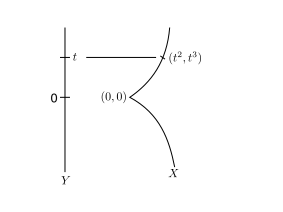
\includegraphics{vol36-figures/fig36-2.eps}}
      \end{figure}
  \end{enumerate}
\end{remarks*}

\section{Divisors, Invertible Sheaves and Line Bundles}\label{chap1:sec2}%sec 2
 
 a)~\pageoriginale  Let $X$ be an irreducible algebraic variety over an
 algebraically closed field $K$, which is locally factorial (i.,each
 $\mathscr{O}_{x}, (x \in X)$ is factorial; this will be the case, for
 instance, if $X$ is non-singular). We denote by $\mathscr{O}$ the
 structure sheaf of $X$ and by $\mathscr{K}$ the constant sheaf of
 rational functions on $X$.   
 
 If $W$ be an irreducible subvariety of $X$, of codimension $1$, then
 $\mathscr{O}_{W}$ is a normal local ring of dimension $1$ and thus is
 $a$ discrete valuation ring; $\mathscr{O}_{W}$ then defines $a$
 discrete valuation on $K(X)$ which we denote by $v_{W}$. 
 
\setcounter{defn}{0}
\begin{defn}\label{chap1:sec2:def1} %defin 1
  $A$ {\em divisor} on $X$ is an element of the free abelian group
  generated by irreducible subvarieties $W$ of codimension $1$ in
  $X$. 
\end{defn}  

Thus a divisor $D$ on $X$ can be written as $D = \sum n(W).W$ with
$n(W) \in \mathbb{Z}$, almost all $n(W)$ being zero.  

If $f$ is $a$ rational function on $X$ then $v_{W}(f) = 0$ for almost
all irreducible subvarieties of codimension $1$ in $X$; in fact if $U$
and $U'$ are the domains of definition of $f$ and $f^{-1}$
respectively, then $v_{W}(f) \neq 0 \Longleftrightarrow W$ is
contained in $(X - U \cap U')$. Therefore $f$ defines $a$ divisor
$(f)=\sum\limits_{W} v_{W}(f)W$ on $X$; such divisors are called
\textit{principal divisors.} 

 The quotient group $\mathcal{D}/_{\mathcal{P}}$ of the group of
 divisors $\mathcal{D}$ on $X$ by the group of principal divisors
 $\mathcal{P}$ on $X$ is called the \textit{Picard group Pic $X$} or
 the \textit{group of divisor classes} on $X$. We say that two
 divisors $D$ and $D'$ are \textit{linearly equivalent} $(D \sim D')$
 if $(D - D')$ is principal.   
 
\begin{defn}\label{chap1:sec2:def2}% defin 2
  An\pageoriginale {\em invertible sheaf} on $X$ is a coherent sheaf of
  $\mathscr{O}$-modules, which is locally free, of rank
  $1$. equivalently it is a coherent sheaf of fractionary
  $\mathscr{O}$-ideals which is locally principal.    
\end{defn}  

\begin{defn}\label{chap1:sec2:def3}%defin 3
  $A$ {\em line bundle} on $X$ is a pair $(L, \pi)$ such that 
  \begin{enumerate}[\rm (i)]
  \item $L$ is an algebraic variety and $\pi : L \to X$ is a morphism
    or simply, a map 
  \item $\exists$ a (finite) open covering $(U_{i})$ of $X$ with $L
    \big|  \pi^{-1}(U_{i}) \xrightarrow{\overset{\varphi_{i}} \sim}
    U_{i} \times K$.  
  \end{enumerate}
\end{defn} 

In the intersections $U_{i} \cap U_{j}$, the isomorphisms
$\varphi_{i}$ and $\varphi_{j}$ define regular maps $g_{i j} :  U_{i}
\cap U_{j} \to K^{*} = K - \{0\}$, such that $g_{i j} .\, g_{j k} =\,
g_{i k}$, in $U_{i}\cap U_{j} \cap U_{k}$ and $g_{ii} = $ identity.  

Conversely, any line bundle is described by giving a finite open
covering $(U_{i})$ of $X$ and regular maps $(g_{ij})$ on the
intersections $U_{i} \cap U_{j}$ to $K^{*}$ with the properties:
$g_{ij}. g_{jk} = g_{ik}$ on $U_{i} \cap U_{j} \cap U_{k}$ and $g_{ii}
= $ identity. The bundle is obtained by ``recollement'' of the varieties
$U_{i} \times K$ through the biregular maps  
\begin{align*}
  (U_{i} \cap U_{j}) \times K & \to (U_{j} \cap U_{i}) \times K \\
  (x,t) & \mapsto (x, g_{ij}(x)  t).
\end{align*}      
 
 We shall now show, by a series of constructions and reverse
 constructions, that the three notions we have define above are
 equivalent. 

\begin{enumerate}[(i)]
\item {\bf Divisor to a Bundle.}\pageoriginale

Since we have assumed $X$ to be locally factorial, any irreducible
subvariety $W$ of codim.$1$ is locally defined by a single equation
(in a $u.f.d$, any prime ideal of height $1$ is principal) and thus
any divisor $D$ is locally principal. We therefore get a covering
$(U_{i})$ of $X$ such that on $U_{i}, D = (z_{i})$ for some $z_{i} \in
K(X)$. If we define $g_{ij} = z_{i}/_{z_{j}}$ or. $U_{i} \cap U_{j}$
then all our requirement are satisfied and we get a line bundle
defined by the $(U_{i}, g_{ij})$.   

\item{\bf Bundle to a sheaf}.

Let $L \xrightarrow{\pi} X$ be a line bundle on $X$. For any open set
$U$ in $X$ a \textit{section} of $L$ over $U$ is by definition a map
$U \xrightarrow{s} L$ such that $\pi o s = $ identity on $U$; these
sections form a group $\Gamma (U,L)$ which is also a $\Gamma
(U,\mathscr{O})-$ module in a natural way. As the fibres $\pi^{-1}(x)$
are $K$-vector spaces of rank $1$, these modules are locally free of
rank $1$ and we thus get an invertible sheaf. 

\item {\bf Sheaf to a Divisor}.

If $\mathscr{L}$ is a locally free $\mathscr{O}-$ module of rank $1$,
we choose an imbedding $\mathscr{L}\hookrightarrow \mathscr{K}$; at any
points $P \in X, \mathscr{L}_{P}$ is a principal fractionary ideal,
say of the form $\mathscr{O}_{P}f, f \in \mathscr{K}_{P} = K(X)$;  for
any irreducible subvariety $W$ of codimension $1$ in $X,\,\, v_{W}(f)
= n(W)$ (say); then $n(W)$ depends only on the imbedding $\mathscr{L}
\subset \mathscr{K}$ and not on the choice of $f$ and again one see that
almost all $n(W)'$are zero. One then associates to $\mathscr{L}$, the
divisor $\sum \limits _{w} n (W) W$.  

We\pageoriginale remark that in (i) if we had started with a $D' \sim D$ oven then
we would have arrived at the same line bundle; and in (iii) if we
had choosen a different imbedding $\mathscr{L} \subset \mathscr{K}$
then we would have arrived at an equivalent divisor. Thus, what we have
shown is that giving an element of Pic $X$ is equivalent to giving a
line bundle or an invertible sheaf.  

\item{\bf Bundle to a divisor}.

In a manner similar to the one defining a line bundle on $X$, we may
define a projective line bundle on $X$ whose fibres are projective
lines $\mathbb{P}_{1}(K)$. By fixing a ``point at $\infty$'' on
$\mathbb{P}_{1}(K)$, hence giving an imbedding $K \hookrightarrow
\mathbb{P}_{1}(K)$, we get an imbedding of a line bundle $L$ on $X$ in
a projective line bundle $\mathbb{P}$ on $X$. If $U$ is an open set in
$X$ and  $s$ is any section of $L$ over $U$, different from the 
``O-section'' $S_o$ or the ``$\infty$-section'' $s_{\infty}$ of $\mathbb{P}$,
take $T = \overline{s (U)} \subset \mathbb{P}$. Then the intersection
cycle $T\cdot (s_o - s_{\infty})$ (see \S 4) is of codimension 2 in $L|U$, and
its projection $\pi (T\cdot (s_{o} - s_{\infty}))$ is of codimension $1$ in
$U$ and therefore determines a divisor $D$ on $U$.    
 
\item {\bf Sheaf to a Bundle}.

Let $\mathscr{L}$ be an invertible sheaf, and $P$ a point on $X$. Then
$\exists$ a section $z$ of $\mathscr{L}$ over a neighbourhood $U$ of
$P$ such that for any $P' \in U', z_{P'} = z(P')$ generates
$\mathscr{L}_{P'}$. We thus take a covering $(U_{i})$ of $X$ and
sections $z_{i} \in \Gamma (U_{i}, \mathscr{L})$ such that $z_{i}$
generates $\mathscr{L}\big|{U_{i}}$; as $z_{i}$ and $z_{j}$ both
generate $\mathscr{L}$ on $U_{i} \cap U_{j}. \, g_{ij} =
z_{i}/_{z_{j}}$ defines a regular map $U_{i} \cap U_{j} \to K^{*}$ and
we thus find a bundle.  

\item{\bf Divisor to a sheaf}.\pageoriginale

Let $D = \sum\limits_{W} n (W) \,W$ be a divisor. For any open subset
$U$ of $X$, we define  

$\mathscr{L}_{D}(U) = \big\{f \in K (X) : v_{W}(f) \ge -n (W)
~\text{for all}~ W ~\text{with}~ W \cap U \neq \phi\big\}$. 

Then $\mathscr{L}_{D}$ is a presheaf on $X$; and if $U$ is open set
such that $D = (g)$ on $U$ for some $g \in K(X)$ then it is easily
checked that $\mathscr{L}_{D}(U)$ is precisely $ = \big\{ f \in K(X) :
f g \in \mathscr{O}_{P} \forall P \in U\big\}$ hence is free on
$\Gamma (U, \mathscr{O})$ of rank $1$, The sheaf $\mathscr{L}(D)$
defined by $\mathscr{L}_{D}$ is thus invertible.  

\item{\bf Certain observations:}

$\alpha)$~ If $D,D'$ are divisors, corresponding to line bundles $L,L'$
  and invertible sheaves $\mathscr{L}(D), \mathscr{L}(D')$ then $D +
  D'$ corresponds to the line bundle $L \underset{X}\otimes L'$ and
  the invertible sheaf $\mathscr{L}(D) \underset{\mathscr{O}}\otimes
  \mathscr{L}(D')$; and $- D$ corresponds to the dual bundle $L^{*}$
  and the dual sheaf $\mathscr{L}(D)^{*}$. 


In fact if $L$ is given by $(U_{i}, g_{ij})$ and $L'$ by $(U_{i},
g'_{ij})$ then $L\underset{X}\otimes L'$  is given by $(U_{i},
g_{ij}.g'_{ij})$ and $L^{*}$ by $(U_{i}, g^{-1}_{ij})$.  

$\beta)$ Let $u : X' \to X $ be a morphism of nonsingular (or locally
factorial) irreducible varieties $X' ,X$. Let $D$ be a divisor on $X$
corresponding to a line bundle $L$ and a sheaf $\mathscr{L}$; then the
``pull-backs'' $u^{*}(L)$ and $u^{*}(\mathscr{L})$ are both well-defined
but where is no way of assuring that $u^{-1}(D)$ is always
well-defined. But one can prove that $\exists$  a divisor $D_{1}\sim
D$ on $X$ such that $u^{-1}(D_{1})$ is (see \S 4) well-defined. Then $u^*
(\mathscr{L})$ and $u^{-1} (D_1)$ correspond to one another. 

$\gamma)$~ Suppose\pageoriginale $L \xrightarrow{\pi} X$ is a line bundle on $X$, and
assume it admits global sections $s_{o},\ldots,s_{n}$ on $X$. Then the
$s_{i}$ are rational functions on $X$ and if we suppose that they do
not vanish (as functions on $X$) all together at any point on $X$, for
every $P \in X$, each ratio $s_{i}(P)/_{s_{j}(P)}$ is either in $K$ or
is $\infty$ in $\mathbb{P}_{1}(K)$. Then the $s_{i}$ define a morphism  
\begin{align*}
  X & \to \mathbb{P}_{n}(K)\\
  P & \mapsto \text{the point given by the homogeneous coords}. (s_{i}(P)).
\end{align*} 
\end{enumerate}

If the $s_{i}$ do have common zeros, then we get only a rational map on $X$
with values in $\mathbb{P}_{n}(K)$. 

\begin{defn}\label{chap1:sec2:def4}%defin 4
  We say that the line bundle $L$ is {\em very ample} if there exist
  an integer $n$ and global sections $s_{o},\ldots,s_{n}$ of $L$ over
  $X$ giving {\em an isomorphism} of $X$ on an algebraic subvariety of
  $\mathbb{P}_{n}(K)$. We say that $L$ is {\em ample} if $\exists$ a
  $q > O$ such that $L^{\otimes q}$ is very ample. We say that a
  divisor $D$ on $X$ is very ample (resp. ample) if the line bundle
  $L_{D}$ defined by $D$ is so. 
\end{defn}  

For any divisor $D$ on $X$ take global sections $f_{o},\ldots, f_{n}$
of the sheaf $\mathscr{L}_{D}$ defined by $D$; they are rational
functions of $X$ such that $(f_{i})+ D \ge 0$ and correspond to global
sections of the line bundle $L_{D}$ defined by $D$. As before we get a
rational map $\varphi_{D}$ of $X$ with values in $\mathbb{P}_{n}(K) ;
\varphi_{D}$ is a morphism if the divisors $(f_{i})+D$ have no common
point. If in 
addition, we assume that the $(f_{i})$ are such that the $\varphi_{D}$
they define is an imbedding of $X$ in $\mathbb{P}_{n}(K)$, then the
divisors $(f)+D$ on $X$ correspond\pageoriginale on $\varphi_{D}(X)$ to the
hyperlane sections for all $f \in \Gamma (X,\mathscr{L}_{D})$. 

\setcounter{proposition}{0}
\begin{proposition}\label{chap1:sec2:prop1}%propo 1
  Let $D,E$ be divisors on $X$ and suppose $D$ very ample. Then $\exists
  n_{o} \in \mathbb{Z}^{+}$ such that for any $n \ge n_{o}$, the sheaf
  $\mathscr{L}(E+n D)$ admits a finite number of global sections,
  defining a morphism $\varphi (E+n D)$  on $X$ into a projective
  space.  
\end{proposition} 
 
\begin{proof}%proof
  We may assume $X$ imbedded in a $\mathbb{P}_{s}$ and that $D$ is a
  hyperplace section. Let $(\xi_{o},\ldots ,\xi_{s})$ be a system of
  homogeneous coordinate in $\mathbb{P}_{s}$ and consider the affine
  open subset $U_{i} \equiv (\xi \neq 0)$ in $X$. The $E \big|{U_{i}}$
  corresponds to a fractionary ideal of $K[U_{i}]$; a finite system of
  generators of the ideal gives a finite system $(s_{ij})$ of sections
  of the line bundle $L_{E}\big| U_{i}$, without a common zero on
  $U_{i}$. Then these sections extend to rational sections
  $(\bar{s}_{ij})$ of $L_{E}$ with poles only on $\xi_{i} = 0$.  

  If  $n(i)$ is the maximum of the orders of these poles then for $n
  \ge n_{i}$ the $(\bar{s}_{ij} \otimes \xi^{n}_{i})_{j}$ are sections
  of $L_{E} \otimes L_{n D} = L_{E+nD}$ on $X$ without common zeros on
  $U_{i}$. Then for $n \ge \underset{i}\sup~ n(i)$ the
  $(\bar{s}_{ij}\otimes \xi^{n}_{i})_{i, j}$ are sections of
  $L_{E+nD}$ without common zeros and hence define a morphism
  $\varphi_{(E+nD)}$ from $X$, into a projective space. \hfill
  \textit{Q,E,P}   
\end{proof} 
 
\begin{proposition}\label{chap1:sec2:prop2}% propo 2
  If $F$ is an ample divisor then $\exists$ a $k_{o} > 0 $ such that
  for any $k \ge k_{o}$, there exist global sections (finitely many)
  of $\mathscr{L}_{kF}$ defining a morphism $\varphi_{kF}$. 
\end{proposition}

\begin{proof}%proof
  By definition some $q{F}$ is very ample. Now apply
  Proposition~\ref{chap1:sec2:prop1} to $D
  = q{F},\, E = F, 2F, \ldots, qF$. 
\end{proof}

\begin{proposition}\label{chap1:sec2:prop3}% propo 3
  If\pageoriginale $D$ is ample then $\exists n_{o} > 0$ such that $nD$ is very
  ample $\forall n \ge n_{o}$.  
\end{proposition}

\begin{proof}%proof
  Some $qD$ is very ample; also choose $k_{o}$ as in
  Proposition~\ref{chap1:sec2:prop2} 
  and $n_{o} = q+k_{o}$. 
\end{proof}

For $n \ge n_{o}, \exists $ a morphism $\varphi_{(n-q)D}: X \to
\mathbb{P}_{\gamma}$ defined by global sections $(f_{i})$ of
$\mathscr{L}_{n-q/D} $; and we have an imbedding  

$\varphi_{qD}: X \to \mathbb{P}_{s}$ defined by global sections
$(g_{j})$ of $\mathscr{L}_{qD}$. Therefore the morphism $\varphi =
(\varphi_{(n-q)D}, \varphi_{qD}): X \to \mathbb{P}_{\gamma} \times
\mathbb{P}_{s}$ is an imbedding (its composite with the projection is
an imbedding); composing with the Segre-imbedding $\mathbb{P}_{r}
\times \mathbb{P}_{s} \to \mathbb{P}_{rs+r+s}$ we get an imbedding
$\varphi_{nD}$ of $X$ in $\mathbb{P}_{rs+r+s}$ defined by global
sections $(f_{i}g_{j})$ of $\varphi_{nD}$.  
\hfill {Q.E.D}

\begin{theorem*}[(Grauert)]%theom
  Let $X$ be a normal irreducible algebraic variety over an
  algebraically closed field $K$ and $L \xrightarrow{\pi'} X$ a line
  bundle on $X$ 

  Let $S_{o}$ be the zero section of the dual bundle $L^{*}
  \xrightarrow{\pi} X$. Then $L$ is ample $\Longleftrightarrow \exists$ 
  a morphism $t$ from $L^{*}$ on an affine variety $Z$ passing through
  the origin in some $K^{n}$ such that    
  
 {\rm (i)}\quad  $t(S_{o}) = 0$
  
 {\rm (ii)} \quad  $L^{*}- S_{o} \xrightarrow{\overset{t}{\sim}} Z - (0)$.
\end{theorem*}

For proving the theorem we shall need the following two lemma.

\begin{lemma}\label{chap1:sec2:lem1}%lamma 1
  Let $L$ be a line bundle on $X$ and $L^{*} \xrightarrow{\pi} X $ the
  dual of $L$. Suppose $s_{o},\ldots,s_{n}$ are sections of $L$ on
  $X$. One then defines a map $\tilde{s}: L^{*} \to K^{n+1}$ by $x \in
  L^{*} \mapsto \tilde{s} (x) = ( \langle s_{i} (\pi(x)), x\rangle)_{i=0}^{n}$. 
\end{lemma}

We\pageoriginale have also seen before that  the $s_i$ define a rational map $s$ on
$X$ to $\mathbb{P}(K)$. We have the following: 
\begin{enumerate}
\item[a)] $\tilde{s} (L^*)\subset$ the affine cone in $K^{n+1}$ of
  $s(X)$, and if $\lambda \in K,\tilde{s}(\lambda x)= \lambda \tilde{s}
  (x)$ 
\item[b)] Any regular map $u: L^* \to K^{n+1}$ such that $u(\lambda
  x)=\lambda \, u(x), \lambda \in K, x \in L^*$ is of the form
  $\tilde{s}$ for a system of sections $s_0,\ldots,s_n$ of $L$. 
\item[c)] Let $S_o$ be the image of the zero section of $L^*$. Then s
  is a biregular imbedding of $X$ in $\mathbb{P}_n(K) \Leftrightarrow
  \tilde{s}$ is biregular outside $S_o \text{ on }L^*$. 
\end{enumerate}

\begin{proof}%proof
  \begin{enumerate}
  \item[a)] The former assertion is clear, for if $\tilde{s}(x)\neq 0,
    \text{ say }\tilde{s}(x)_o\neq 0$, then, for each
    $\dfrac{\tilde{s}(x)_i}{\tilde{s}(x)_o}=\dfrac{s_i(\pi(x))}
         {s_o(\pi(x))}$ ; the latter assertion is trivial. 
  \item[b)] Let $ u(x)=(u_o(x),\ldots ,u_n(x)), x \in L^*$. For any $a
    \in X$  if  $x \in (L^*)_a \text{ then }x \to u_i(x)$ is a linear
    form on $L^*_a$ and thus defines an $s_i(a) \in (L^*)^*=L_a$; and
    therefore we get sections $s_i\in \Gamma(X,L), 0 \leq i \leq n$ with the
    required property. 
  \item[c)] Assume $s:X \to \mathbb{P}_n$ is a biregular
    imbedding. Let $x \in L^*-S_o$ and  $a\in X \text{ s. t } x \in
    L^*_a$; if $i$ is such that $s_i(\pi (x))\neq 0 $ then
    $\tilde{s}(x)_i \neq 0 \text{ and } \tilde{s}(x) \neq
    0$. Therefore $\tilde{s}(L^*-S_0) \subset \{\text{cone of}~ s(X)-(0)\}$
    in $K^{n+1}$. We will prove that this inclusion is, in
    fact, an equality; it is sufficient to prove our assertion when we
    restrict $L^*$ to an open at $U \ni a \text{ in }X \text{
      s-t}. L^*$ over $U$ is isomorphic to $U \times K$. Then $L^* -S_o
    \simeq U \times K^*$, while, the cone of $s(U)-\{0\}$ is
    isomorphic to $s(U) \times K^*$. 
\end{enumerate}
\end{proof}

As\pageoriginale all these isomorphisms are compatible with restrictions of $U$ to
smaller open sets, we are through, we have, by hypothesis, $U
\xrightarrow{\sim}  s(U)$ 

Conversely,let $s(L^*-S_o) \xrightarrow{\sim} \tilde{s}(L^*)-\{0\}$;
again by choosing an open $U \subset X$ such that $L^* \simeq U
\times K$ we get  

$ U \times K^* \xrightarrow{\sim}  s(U) \times K^*$ by an isomorphism
compatible with restrictions and identity on $K^*$  i. e., $U
\xrightarrow{\sim} s(U))$; and $s$ is thus a biregular imbedding of
$X \text{ in } \mathbb{P}_n $.  

\begin{lemma}\label{chap1:sec2:lem2}%lamm 2
  Let $E$ be a line bundle on $X$ and $v_q$ be the morphism of fibre
  spaces $E \xrightarrow{v_q} E^{\otimes q}$ on  $X$, defined by  
  $$
  x \to x \otimes \cdots \otimes x, (q ~\text{times}).
  $$
\end{lemma}

Suppose $u$ is any morphism $E \to K^n$ such that $u(\lambda x)
=\lambda^q u(x). \lambda \in K, x \in E$. Then $u$ admits a unique
factorization  
$$
E \xrightarrow{v_q} E^{\otimes q}\xrightarrow{\bar{u}} K^n
$$
such that $\bar{u}$ is a morphism with $\overline {u}(\lambda x) =
\lambda \overline {u}(x), x \in E^{\otimes q},\lambda \in K$. 

\begin{proof}%proof
  Is $x,y \in E \text{ are s.t. } v_q(x)=v_q(y) \text{ then } y=
  \alpha x, \alpha \in K$. 
  Also, $v_q(y)=(y \otimes \cdots \otimes y) =\alpha^q (x \otimes
  \cdots \otimes x)= x \otimes \cdots x = v_q (x)$ by assumption so
  that $\alpha$ is a $q^{th}-$ root of unity. Then $u(y)= \alpha^q
  u(x)$ by hypothesis, and so $u(y)=u(x)$ so that the set theoretic
  map $\overline {u} \text{ on } E^{\otimes q}$ defined by  
  $$
  \overline {u}(v^q(x))=u(x) \text{ is }\textit{well-defined}.
  $$
  To show that $\overline {u}$ is a morphism take any open $U \subset X$
  such that $E|U \simeq U \times K$ and $E^{\otimes q}|U \simeq U
  \times k$. If $(x)=(z,\lambda)$ is a coordinate system for $E|U$ and
  $(x')=(z', \mu)$ 
  a coordinate system for $E^{\otimes q}|U$ then $v_q$ is given by
  $(z,\lambda) \to (z,\lambda^q)$ and $\overline {u}$ is given by
  $\overline{u} (z', \mu) = \overline {u}(z',1).\mu =u(z',1)\mu$
  \hfill{Q.E.D.} 
\end{proof}

\subsubsection*{Proof of Grauert's theorem}\pageoriginale

\textbf{(i)  Necessity}

If $L$ is ample by Proposition~\ref{chap1:sec2:prop3}, $\exists q>0$ and systems of
sections $(s)$ of $L^{\otimes q} \text{ and } (s') \text{ of
}L^{\otimes(q+1)}$ defining projective imbeddings  
$$
\displaylines{\hfill  s: X \to \mathbb{P}_n \hfill \cr
\text{ and }\hfill  s': X \to \mathbb{P}_n' \text{
  respectively}.\hfill }
$$

As in Lemma~\ref{chap1:sec2:lem1}, we obtain morphisms
$$
\tilde{s}:(L^*)^{\otimes q} \to K_{n+1} \text{ and }
\tilde{s}:(L^*)^{\otimes}\xrightarrow{(q+1)} K_{n'+1} 
$$
which are biregular imbeddings outside the respective null sections 
\break (Lemma~\ref{chap1:sec2:lem1}, c). We define now a morphism $v: L^* \to K_{n+n'+2}$ as the
composite  
$$
L^* \xrightarrow[v_q \oplus v_{q+1}] {} (L^*)^{\otimes q} \oplus
(L^*)^{\otimes(q+1)} \xrightarrow[\tilde{s} +\tilde{s}'] {}
K_{n+n'+2}. 
$$

We shall prove the $v$ is a biregular imbedding outside the null
section $S_o \text{ of }L^*$. It is enough to show that $v_q \oplus
v_{q+1}$ is a biregular imbedding outside $S_o$. Again it suffices to
do this over open sets $U \subset X$ such that $L^*|U \simeq U \times
K$; over $U$ the map $v_q \oplus v_{q+1}$ is given by $(x,\lambda)
\mapsto (x,\lambda^q) \oplus(x,\lambda^{q+1})$; the inverse rational
map form the image is given by $(x,t) \oplus (x,t') \mapsto (x,t'/_t)
; v_q \oplus v_{q+1}$ is then certainly a biregular imbedding on $(L^*
-S_O)|U \simeq U \times K^*$.  

\medskip
\noindent \textbf{(ii)  Sufficiency.}

Let $t$ be a morphism on $L^*$ with the properties stated in the
theorem.\pageoriginale For any $x \in L^*$ one obtains a map $K \rightarrow K^n
\text{ by } \lambda \mapsto t(\lambda x)$: this is defined on the
whole of $K$ and vanishes precisely for $\lambda=0 \text{ or } x \in
S_o$. Hence there exist regular maps $t_1(x),\ldots,t_r(x) $ on $L^*$
to $K^n$ such that  
$$ 
t(\lambda x)=\lambda t_1(x)+\cdots + \lambda^r t_r(x).
$$

Computing $t(\mu \lambda x)$ we easily see that $t_j(\mu x)=\mu^j
\,t_j(x) \forall\underset{\mu \in K} {x \in L^* }$. The map
$t(x)=t_1(x)+\cdots + t_r(x)$ is an imbedding of $(L^* -S_o)$; thus
the map $u(x)=(t_1(x),\ldots , t_r(x)) \text{ of } L^*$ in a suitable
big affine space is also an imbedding outside $S_o$. 

Let $t_{jk}( x)$ be the components of the map $t_j(x)$; we have
$t_{jk}(\mu x)=\mu^j t_{jk}(x) \forall \mu \in K, x \in L^*$. We form
the graded ring  $ A=K\left[(t_{jk)_{j,k}}\right]$, the degree of
$t_{jk}$ being $j$. Then $A$ is a domain (it is the coordinate ring of
the image $u(L^*))$; its integral closure $A'$ is a graded, finite
type $K$-algebra. Then $\exists~ q<0$ such that the homogeneous elements
in $A'$ of degree $q$ generate $A'(q)=\sum \limits_{\nu \geq 0}A'_{\nu
  q}$ as a graded $K$-algebra; we may assume $q$ to be a multiple of
$1,2,\ldots,r$. Let $(w_{\alpha})$ be a basis over $K$ of the $K$-space
$A'_q$; $(w_{\alpha})$ are regular functions $L^* \to K$, homogeneous
of degree $q$. We obtain then a regular map $w:L^* \to K^N \text{ for
  an }N \in \mathbb{Z}^+ $ whore components are the $(w'_{\alpha})$s and
which therefore has the property $w(\lambda x)=\lambda^q w(x),x \in
L^* ,\lambda \in K $. By Lemma~\ref{chap1:sec2:lem2}, we get a factorization  
$$ 
L*\xrightarrow{v_q} (L^*)^{\otimes q} \xrightarrow{\bar{w}} K^N
$$
such\pageoriginale that $\overline{w}(\mu y)=\mu \overline{w}(y),y \in
(L^*)^{\otimes q},\mu \in K$.We shall prove that $(L)^{\otimes q}$ is
\textit{very ample} by showing that $\overline{w}$ is an imbedding
outside its null section (see Lemma 1,c)). 

As $\overline{w}((L^*)^{\otimes q})=w(L^*)$ is a \textit{normal}
subvariety of $K^N$ (its coordinate ring is $K[(w_{\alpha})]$ we shall
prove our ascertain by using Zariski's main theorem (Chapter $I$,
$g$)) i.e. by proving that $\overline{w}$ is bijective, birational
onto its image, outside $S_\circ((L^*)^{\otimes q})$. 


\noindent{\bf {\boldmath $\overline{w}$ is injective outside
    $S_o((L^*)^{\otimes q})$}:}
\begin{enumerate}
\item[a)] If $w(x)=w(y), \text{ then }\exists \text{ a } q^{th}$ root
  of unity $\varepsilon$ such that $t_{jk}(y)=\varepsilon^j t_{jk}(x)
  \forall j, \mathcal{R}$. 

  In fact, each $t^{q/j}_{jk}$ is a linear combination of the $w'_
  {\alpha}$ $s$ so that $w(x)=w(y) \text{ implies
  }t^{q/j}_{jk}(x)=t^{q/j}_{jk}(y)$, 
  $$
  \text{ i. e} \qquad t_{jk}(y)=\varepsilon_{jk}t_{jk}(x)
  $$
  where $\varepsilon_{jk}$ is a $(q/j)^{th}$root of unity. In
  particular, $\varepsilon=\varepsilon_{11}\text{ is a }q^{th}$ root
  of unity. Now $t_{jk}t^{q-j}_{11}$ is again a linear combination of
  the $w'_{\alpha}$s and therefore  
  $$
  \displaylines{\hfill 
  t_{jk}t^{q-j}_{11}(y) = t_{jk}t^{q-j}_{11}(x)\hfill \cr
  \text{i.e.,}\hfill 
  \varepsilon_{jk}\varepsilon^{q-1}t_{jk}t^{q-j}_{11}(x)=t_{jk}t^{q-j}_{11}(x)\hfill
  }  
  $$
  and for $x \notin S_o$, this means $\varepsilon_{jk}=\varepsilon^j$.

\item[b)]Suppose\pageoriginale $x',y' \in (L^*)^{\otimes q}$ such that
  $\overline{w}(x')=\overline{w}(y')$. 
\end{enumerate}

Let $x'=v_q(x), y'=v_q(y), \text{ with }x,y \in L^*$. Then by a) we
obtain  $t_{jk}(y)=\varepsilon^j t_{jk}(x)=t_{jk}(\varepsilon \,x)
\forall j, k$. This implies $t(y)=t(\varepsilon x)$ for the
map $t=t_1 +\cdots +t_r$; but if $x',y'\in (L^*)^{\otimes
  q}-S_o((L^*)^{\otimes q})\text{ then } x,y \in L^* -S_o\text{ and }
t$ is biregular on $L^*-S_o$ by hypothesis. Therefore $y=\varepsilon x
\text{ and } y'=v_q(y)=\varepsilon^q v_q(x)=x'$. 

\medskip
\noindent {\bf{\boldmath  $\overline{w}$} is birational} 

We have $K(L^*)= K((t_{jk})_{j,k})$; the projection $\pi:L^* \to X$
then gives an imbedding $K(X) \hookrightarrow K((t_{jk}))$. As locally
$L^*$ is of the form $X \times K$, this means that $\exists$ a
homogeneous function $\sigma \in K(L^*)$ of $\deg$  1,
$\sigma(\lambda x)=\lambda \sigma (x)$, such that
$K(L^*)=K(X)(\sigma)$. Obviously, then $K((L^*)^{\otimes q}) =\break K(X)
(\sigma^q)$. 

On the other hand, $K(X)$ is generated over $K$ by the elements in
$K((t_{jk}))$ which are products of the form $\prod\limits_{j,k}
t_{jk}^{\beta^{(j,k)}}\text{ with } \sum \limits_{j,k}
\beta(j,k)=0$. Thus $K(X)=K((w_{\alpha}/_{w_{\alpha_o}}\big)_{\alpha}
)$ and the function field $F$ of $\overline{w}((L^*)^{\otimes
  q})$ is given by  
$$
F=K((w_{\alpha})_{\alpha})= K(X)(w_{\alpha_o}).
$$

Finally as  $\sigma^q /w_{\alpha_o} \in K(X)$, we obtain 
\begin{equation*}
  F=K(X)(\sigma^q)=K((L^*)^{\otimes q)}.\tag*{Q.E.D}
\end{equation*}

\section{Chow Coordinates}\label{chap1:sec3}%sec 3

a)~\pageoriginale Let $V$ be an algebraic set of dimension $d$ in $\mathbb{P}_n$
(notation: $V^d$); we assume that $V$ is pure of dimension $d$, i.e., all the
components of $V$ have the same dimension $d$. If $H_1$ is a hyper
plane not containing any component of $V$ then $H_1 \cap V$ is pure of
dimension $(d-1)$. If $H_2$ is a hyperplane not containing any
component of $H_1 \cap V \text{ then } H_2 \cap H_1 \cap V$ is pure of
dimension $(d-2)$ and so on; and finally $H_{d+1}\cap \cdots \cap H_1 \cap V$
is empty \textit{ in general}. 

Our purpose now is to study the systems of $(d+1)$ hyperplanes
$H_o,\ldots, H_d$ such that $(H_o\cup \cdots \cap H_d) \cap V $ is \textit{
  non-empty}. 

Assume $V$ to be irreducible. Any hyperplane $H$ will be defined by an
equation of the form $\sum \limits^n_{i=0}u_i X_i=0 \text{ in
}\mathbb{P}_n, u_i \in K$ and is there fore determined by the point
$(u_o, \ldots ,u_n ) \in K^{n+1}$. A system of $(d+1)$ hyperplanes
will then be determined by a point in the affine space
$K^{(n+1)(d+1)}$. We shall now prove that the points in
$K^{(n+1)(d+1)}$ corres ponding to systems of (d+1) hyperplanes $H_P,
\ldots, H_d \text{ in } \mathbb{P}_n$ such that $V \cap H_O \cap
\cdots \cap H_d \neq \phi $ form an irreducible algebraic variety (in
fact, a cone for obvious reasons ) in $K^{(n+1)(d+1)}$. 

Let $k$ be a field of definition for $V$ and $(x)=(x_1, \ldots,x_n)$
be the affine coordinates for a generic point $(x)$ of $V/k$. Its
homogeneous coordinates are the $(1,x_1, \ldots,x_n)$. Consider a
system   
$$
\overline{u}_{ij},i=0,\ldots,d, \, j=1, \ldots, n
$$
of algebraically independent elements of $K$ over $k(x)$ and an equation
$$
\overline{u}_{io}=-\sum^n_{j=1} \overline{u}_{1j}x_j \qquad \text{
  defining } (\overline{u}_{io})_{i=0, \ldots,d} 
$$

Then\pageoriginale $(\overline{u}_{ij})$ is a generic point of an irreducible
variety in $K^{(n+1)(d+1)}$ (the locus of $(\overline{u}_{ij})$ over
$k(x)$ which is the one we have been looking for. Its dimension is
$d+ n(d+1)= n(d+1)(d+1)-1$ so that it is a hypersurface in $K^{(n+1)(d+1)}$,
defined by an equation:  
$$
F(u_{oo}, \ldots ,u_{on}; u_{1o}, \ldots , u_{1n} ; ---- ; u_{do,
  \ldots , u_{dn}})=0 
 $$ 
in $(n+1)(d+1)$ variables; this equation is obviously multi homogeneous
in the set of variables indicated, of the same degree $\delta$, in
each set of variables; if two sets of variables take the same values
then the hyperplanes they define are the same and $H_o \cap \cdots
\cap H_d \cap V \neq \phi$ in valid; this implies that $F$ is
containing and antisymmetric in the sets of variables indicated. 

The polynomial $F$ is called the \textit{Chow form} (or the associated
form, or the Cayley form or the Bertini form)of $V$. 

The Chow form $F(V)$ of a variety $V^d$ determines the variety $V$
back uniquely. In fact for any  linear variety $L^{n-d}$ the points of
intersection of $L^{n-d}$ and $V$ are given by the Chow form F(V) and
are precisely $\delta=$ degree of $F(V)$, in number.$\delta$ is called
the \textit{degree of the variety} $V$. 

b) Let $V$ be any variety. By a \textit{cycle} on $V$ we mean an
element of the free abelian group generated by irreducible subvarieties of
$V$. If $X=\sum n_\alpha V_\alpha$ is a cycle on $V$. the support of
$X$ is the union $\bigcup\limits_{n_\alpha \neq=0}V$. 

We say that $X$ is of dimension $d$ if each  $V_\alpha$ is of
dimension $d$; we say that $X$ is
\textit{positive} $(X \geq 0)$ if each $n_\alpha$ is $\geq 0$. 

If\pageoriginale $X=\sum n_\alpha V_\alpha $ is a positive cycle of dimension $d$
in $\mathbb{P}_n(K)$ and  $F_\alpha (u)$ is the Chow form of each
$V_\alpha$ the form $F(u)=\prod\limits_{\alpha }(F_\alpha (U))^n
\alpha$ is called the \textit{Chow form of the cycle $X$}. The
degree of $F(u)=\sum n_\alpha \deg V_\alpha $ is called the
\textit{degree of the cycle} $X$. We may write Chow form $F(u)$ in the
form $\sum$ $C_\lambda (X)u_\lambda$ where the $u_\lambda$ are monomials; we then call the  $(C_\lambda
(X))$ the \textit{Chow coordinates} of $X$, and the point whose
homogeneous coordinates are the $(C_\lambda (X)_\lambda)$ is called
the \textit{Chow point} of $X$.  

Conversely, if $G(u)=$ $d$ $u$ is a given form multihomogeneous of the
same degree in each set of variables, alternating and antisymmetric,one
may ask ``Under what condition are the $(d)$ the Chow  coordinates of a
positive cycle on a subvariety $U$  $n^?$''.The answer is given by the
following theorem which we shall not prove here. (For a proof see
Chapter I,\S 9,5, Samuel \cite{4}). 

\begin{theorem*}%them
  The $(d_\lambda)$ are the Chow coordinates of a positive cycle $X$
  on a subvariety $U \subset \mathbb{P}_n(K)$ if and only if the
  $(d_\lambda)$ satisfy a system of homogeneous equation with
  coefficients in the smallest field of definition of $U$. 
\end{theorem*}

We call a system of cycles $(X_\alpha )$ an \textit{irreducible}
system if the Chow points of the $X_\alpha $ range over an irreducible
variety. 

\begin{coro*}%cor
  Any system of positive cycles on $\mathbb{P}_n(K)$ with a given
  dimension  $d$ and a given degree $\delta$ is a finite union  of
  irreducible systems. 
\end{coro*}

\begin{example*}%exam
~

  \begin{enumerate}[\rm a)]
  \item {\em $V=\{(a_o,\ldots,a_n)\}$, a point in $\mathbb{P}_n$}.

    The Chow form $F(u)$ of $V$ is the linear form  $\sum
    \limits_{i=1}^{n} u_i a_i=0$. 
  \item $V$\pageoriginale {\em a hyperplane $H$ given by} $\sum \limits_{j=0}^{n}a_j
    X_j=0$. Then the Chow form of $V$ is given by the determinant  
    $$
    \begin{vmatrix}
      a_o & \cdots & a_n\\
      u_{oo} & \cdots & u_{on}\\
      & \cdots &\\
      u_{n-1},o & \cdots & u_{n-1},n\\
    \end{vmatrix}
    =0
    $$
  \item {\em $V$ a linear subvariety of $\mathbb{P}_n$}.
  \end{enumerate} 
\end{example*}

In this case the Chow coordinates are essentially the Grassmann
coordinates of the linear variety. 

\section{Results from Intersection Theorey}\label{chap1:sec4}%sec 4

a)~ We fix, for our present consideration, an ambient variety $U$, over
an algebraically  closed field $K$, which we shall assume to be non
singular. Let $V,W$ be irreducible closed subvarieties of $U$. We say
that   a component $C$ of $V \cap W$ is \textit{proper} if $\dim
C=\dim V+\dim W-\dim U$. For such a component $C$, the
\textit{intersection multiplicity} $i_U(C;V.W)$ is defined in the
following manner: 

Consider the product (nonsingular) variety $U \times U$ and let
$\triangle$ be the diagonal of $U \times U$; then the component $C$
corresponds to a component $\tilde{C}$ of $\triangle \cap (V \times
W);\tilde{C}$ is an irreducible subvariety of $V \times W$ and  if
$\mathscr{O}$ is  local ring of $\tilde{C}$ on $V \times W$ then
$\mathscr{O}\subset K(V \times W)$; then $\triangle \cap (CV \times
W)$ is defined by equations $(X_i-X'_i)$ in  $K[V \times W]$ locally and
these equations generate an ideal $q$ in $\mathscr{O}$, primary for the
maximal ideal of $\mathscr{O}$. \textit{The intersection multiplicity
  of} $V$ \textit{and} $W$ \textit{on} $C$ is defined to be the
multiplicity\pageoriginale $e(q)$ of the primary ideal $q$ in $\mathscr{O}$. 

It can be shown that $i_U(C;V.W)=1$ means that  $\mathscr{O}$ (in the
above paragraph) is a regular local ring and $q$ is the maximal ideal
of $\mathscr{O}$. The first condition means that $C$ is simple on $V$
and $W$: the second condition says precisely that the tangent spaces
to $V$ and $W$ at a generic point of $C$ have for their intersection
the tangent space to $C$ at that point. We say then that  $V$ and $W$
are \textit{transversal} on $C$. 

\begin{remark*}%rem
  We observe that so far we have not made any use whatever of the fact
  that $C$ is a proper component  of $V$  $W$. We could have defined
  $i_U(C;V.W)$ for any component  $C$ of $V \cap W$. But the advantage
  in considering a proper component is seen from the following fact
  (which we shall not prove): 
\end{remark*}

Let $C$ be a proper component  of $V^d \cap W^{d'}$ in a (nonsingular)
$U^n$; suppose that the primary ideal  of $V$ in $\mathscr{O}(C;U)$
(the local ring of $C$ in $U$) is generated by $(n - d)$ elements
$y_1, \ldots , y_{n-d}$ (this  will be the case for  instance if $C$
in simple on $V$); then the multiplicity $i_U(C;V.W)$ is equal to the
multiplicity of the ideal of $\mathscr{O}(C.W)$ generated by the
classes of $(y_i)$. 

(For a proof see Chapter II, \S 5, no.7, Theorem 6), Samuel \cite{4} 

With the same notation,we define the ``intersection'' $V\cdot W$ (or
$\bigcup\limits^{V \cdot W}$ when all the components $C_\alpha$ of $V
\cap W$ are proper, by: 
$$
V.W=\sum i_U (C_\alpha :V.W)C_\alpha 
$$

Then\pageoriginale $V\cdot W$ is a \textit{cycle} on $V \cap W$. Under obvious
condition, we may also define the cycles $\underset{U}{X \cdot Y}$ for
two cycle $X,Y$ on $U$, by extending the above definition by
linearity. When the ambient space $U$ needs no special mention we may
also write $X.Y$ for $\underset{{U}}{X\cdot Y}$. 

\subsubsection*{Some properties}

\begin{enumerate}[i)]
\item 
  $$
  \displaylines{X \underset{{U}}.U  = X  \cr
    \hfill X \underset{{U}}.Y  = Y\underset{U}.X \hfill \cr 
    \qquad \text{and}\hfill 
    (X \underset{U}.Y)\underset{U}. Z  = X\underset{U}.(Y
    \underset{U}.Z)\hfill }
  $$
  (We remark that the associativity holds only when all the component
  of $U \cap V \cap W,(U,V,W$  being the components of  $X$, $Y$, $Z$
  respectively are proper).  
  
\item If $X,Y$ are cycles on $U,X',Y'$ cycles on $U'$ then  $X \times
  X'$ and $Y \times Y'$ are cycles on $U \times U'$, and one has $(X
  \times X')$.$(Y \times Y')=(X.Y)\times (X'.Y')$ 
  
\item Let $V$ be a closed, nonsingular subvariety of $U,X$ a cycle on
  $V,Y$ a cycle $U$ then  
  $$
  X \underset{U}.Y=X \underset{V}.(V \underset{U}.Y) \quad \text{(Induction
    formula)}. 
  $$

\item Let $U,U'$ be nonsingular varieties and $p: U \times U' \to U$ the
  set-theoretic projection. Let $V$ be a subvariety of $U \times U'$; we
  define  the \textit{algebraic projection} $pr_U(V) $ of $V$ as
  follows: 
  \begin{enumerate}
  \item[$\alpha$)] if dim $\overline{p(V)<} \dim V$, then $pr_U(V)$ is
    the ``zero cycle'' on $U$
  \item[$\beta$)]  if $\dim \overline{p(V)}=\dim V$, them $K(V)$ is a
    finite extension of\break $K(\overline{p(V)})$ and $pr_U(V)$ is the cycle $\left[ K(V):K
      \overline{(p(V))}\right]\overline{p(V)}$. 
  \end{enumerate}

  This\pageoriginale notion of an algebraic projection extend by linearity to cycles
  on $U \times U'$. 
\end{enumerate}

\begin{prop*}% propo
  Let $U'$ be a {\em complete} nonsingular variety and $X$ be a cycle
  on $U \times U'$. Then  for any cycle  $Y$ on $U$. 
  $$
  pr_U(X\cdot (Y \times U'))=pr_U(X)\cdot Y
  $$
  whenever both sides are defined. 
\end{prop*}

b)~ Given a morphism $f:V \to V'$ of nonsingular varieties and a cycle
$X'$ on $V'$, one defines the inverse image $f^{-1} (X')$ as $pr_v ((
V \times X')\cdot \Gamma_f)$ where $\Gamma_f$ is the graph of $f$.
 Let $V$ be a projective nonsingular variety and $T$ an irreducible
variety, also  nonsingular. For any cycle  $X$ an $V \times T$, the
cycle $X_t=pr_V((V \times t) \cdot X)$ on $V$ is defined for ``almost
all'' $t \in T$. The system of cycles $(X_t)$ thus defined on $V$ is
said to be an \textit{irreducible algebraic family of cycles on} $V$. 

One can show that for an algebraic family $(X_t)$ of cycles on $V$,
the Chow coordinates $c(X_t)$ of the cycle $X_t$ depend rationally on
$t\in T$:thus the dimension and degree of the cycle $X_t$ are
independent of $t \in T$. Any two members  of the family $(X_t)$ are
said to be \textit{algebraically equivalent}. 

Let $(X_t)_{t \in T}$ and  $(Y_{t'})_{t' \in T'}$ be algebraic
families of cycles on $V$; we may assume that the parametrizing
varieties $T$ and $T'$ are the same by passing  to $T \times T'$ in
the obvious manner. Then it is checked that 
$$
X_t\cdot Y_t=pr_V((V \times t)\cdot (X\cdot Y))
$$
where $X$ and $Y$ are the ``defining'' cycles on $V \times T$. Thus
$(X_t\cdot Y_t)_{t \in T}$ is again an algebraic family on $V$. 

\begin{examples*}%exam
  We\pageoriginale shall be interested here only in cycle of dimension 1,  i.e.linear
  combinations of irreducible curves. 
  \begin{enumerate}
  \item[(i)] Let $D$ and $E$ be cycles of (dimension 1 and) degrees
    $d$ and $e$ in $\mathbb{P}_2$. The intersection number $(D.E)$ of
    $D$ and $E$ is the total number of points of intersection of $D$ and
    $E$  each  point counted with the appropriate multiplicity. 
    
    We have:$(D.E)=de$ (Theorem of Bezoout). In fact , it is enough to
    prove this for cycles $D'$ and $E'$ such that $D$ is  algebraically
    equivalent to $D'$ and $E$ is algebraically equivalent to $F'$. One
    can construct an algebraic family containing $D$ and $D'=dL$($L$ a
    line) as members and similarly for $E$ and $eL'$. For the two lines
    $L$ and $L'$ our assertion is obvious. 
    
    Thus, we have a case where the intersection  number is completely
    determine  by the degrees of the  cycles 
    
  \item[ii)] Consider the products of the projective lines $\mathbb{P}_1
    \times \mathbb{P}_1$ imbedded in $\mathbb{P}_3$. Thus is the quadric
    $\xi_o \xi_1-\xi_2 \xi_3=0 $ in $\mathbb{P}_3$. 
%  \quad
%  \begin{minipage}{5cm}
    \begin{figure}[H]
      \centerline{\includegraphics{vol36-figures/fig36-3.eps}}
    \end{figure}
%  \end{minipage}\qquad 
%  \begin{minipage}{4cm}
    Let $L_1$ and $L_2$ be a `horizontal' and a `vertical' line  of this
    product: if $d_1=(X\cdot L_2)$ and   $d_2=(X\cdot L_1)$ one may
    construct an  algebraic family on $\mathbb{P}_1 \times \mathbb{P}_2$
    containing $X$ and $(d_1L_1+d_2 L_2)$ as members. Similarly  for a
    second cycle $X'$ in $\mathbb{P}_1 \times \mathbb{P}_1$ 

  The\pageoriginale intersection number of the cycles $X,X'$ is then given by 
  \begin{alignat*}{4}
    &&(X \cdot X')&=\bigg
    ((d_1L_1+d_2L_2).(d'_1L_1+d'_2L'_2)\bigg)\hspace{1cm}\\ 
    &&& = d_1 d'_2+d_2d'_1\\
    \text{while} &\hspace{2cm}&\deg X &= d_1+d_2 \quad \text{and}\\
    &&\deg X' & = d'_1+d'_2\\
  \end{alignat*}
  
  We have thus a case where the  intersection number is \textit{not}
  determine by the degrees of the cycles.  
  \end{enumerate}
\end{examples*}

